\chapter{Introduction}\label{chap:intro}
    \textit{Give a short abstract of your chapter here for when your examiner gets bored and wants the tl;dr}
    %
    \begin{center}
      $\bowtie$~$\bowtie$~$\bowtie$
    \end{center}
    %
    Particle physics experiments perform some of the most precise measurements of natural phenomenon in science. 
    Quantities such as the mass of the electron are known within 1 part in 100 trillion\cite{paper:CODATA}.
    \section{Understanding \Bmunu via the Standard Model}
        The subatomic physics decay \Bmunu is that of an electrically-charged $B$, a composite particle.
        The $B$ decays to the electron-like particle, a muon ($\mu$), alongside the electrically neutral neutrino ($\nu$), a particle with near zero mass. 
        The process can be drawn as a Feynman diagram, as in \Fig{fig:Bmunu}.
        \begin{figure}[htpb]
            \begin{center}
                \begin{tikzpicture}
                    \begin{feynman}
                        \vertex (u) {\(\u\)}; 
                        \vertex [below right=of u] (v1);
                        \vertex [below left=of v1] (bbar) {\(\bbar\)}; 
                        \vertex [right=of v1] (v2);
                        \vertex [above right= of v2] (mu) {\(\nu_{\mu}\)};
                        \vertex [below right= of v2] (nu) {$\mu^{+}$};
                        \vertex [above left=0.25 and 0.5 of u] (u');
                        \vertex [below left=0.25 and 0.25 of bbar] (bbar');
                        \diagram*{
                            (u) -- [fermion] (v1) -- [fermion] (bbar),
                            (nu) -- [fermion] (v2) -- [fermion] (mu),
                            (v1) -- [photon,edge label={\(W^{+}\)}](v2),
                        };
                        \draw [decoration={brace}, decorate] (bbar') -- (u') node [pos=0.5, left] {\large $B^{+}$};
                    \end{feynman}    
                \end{tikzpicture}
            \end{center}
            \caption{A Feynman diagram of the decay \Bmunu, indicating the effect of Standard Model forces that facilitate this process.}%
            \label{fig:Bmunu}
        \end{figure}
        
        SM theory has also been used to mathematically predict and later experimentally confirm the existence of further ones.
        A complete explanation of the matter, mediator and resulting mathematical mechanisms of SM is not the focus of this thesis, and thus the scope is limited to how SM explains and predicts \Bmunu process.\\ 
        \begin{figure}[htpb]
            \centering
            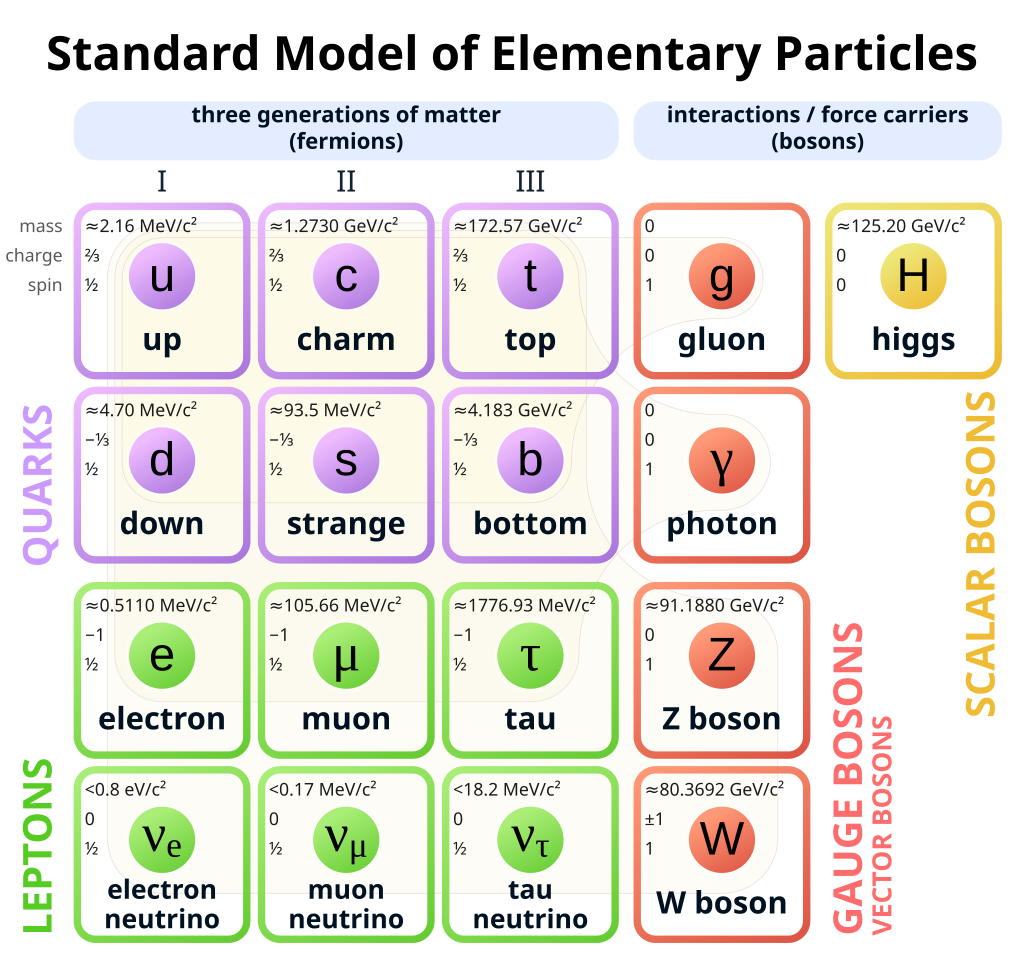
\includegraphics[width=0.62\textwidth]{./Intro/Figures/1024px-Standard_Model_of_Elementary_Particles.svg.png}
            \caption[The twelve fundamental fermions and five fundamental bosons of the Standard Model of Particle Physics. Each particle is uniquely defined by its mass, charge and intrinsic spin.]{The twelve fundamental fermions and five fundamental bosons of the Standard Model of Particle Physics\cite{pic:SM}. Each particle is uniquely defined by its mass, charge and intrinsic spin.} 
            \label{fig:SM}
        \end{figure}
        % Now we talk about pieces
        \subsection{Standard Model Particles and their Interactions}
            \subsubsection{Muons and neutrinos}
                The $\mu$ and $\nu_\mu$ in the final state of \Bmunu are a pair of matter particles referred to as \textit{leptons}.
                As seen in \Fig{fig:SM}, there are six leptons in SM, occurring in three generations of pairs between a neutral and a charged lepton.

\begin{center}
  $\bowtie$~$\bowtie$~$\bowtie$
\end{center}
